\subsection{Discussion}
% -------------------------------------------------------------------------
The novel segmentation method proposed in this work achieves segmented results
that are approximately 7\% more accurate than a typical watershed segmentation
when each are compared with the same manual segmentation.
AN overlay of the mismatched pixels can be used to visualize the improvements
between segmentations more clearly than a simple comparison.
Each segmentation is plotted with red pixels overlaid
indicating mismatched with the manual segmentation.
This visualization represents the higher number of mismatched pixels in the
typical watershed segmentation (\ref{fig/05/seg-comps}.c)
as a higher number of red pixels than in the merged-region segmentation
(\ref{fig/05/seg-comps}.f).

\begin{figure}[ht]
    \centering
    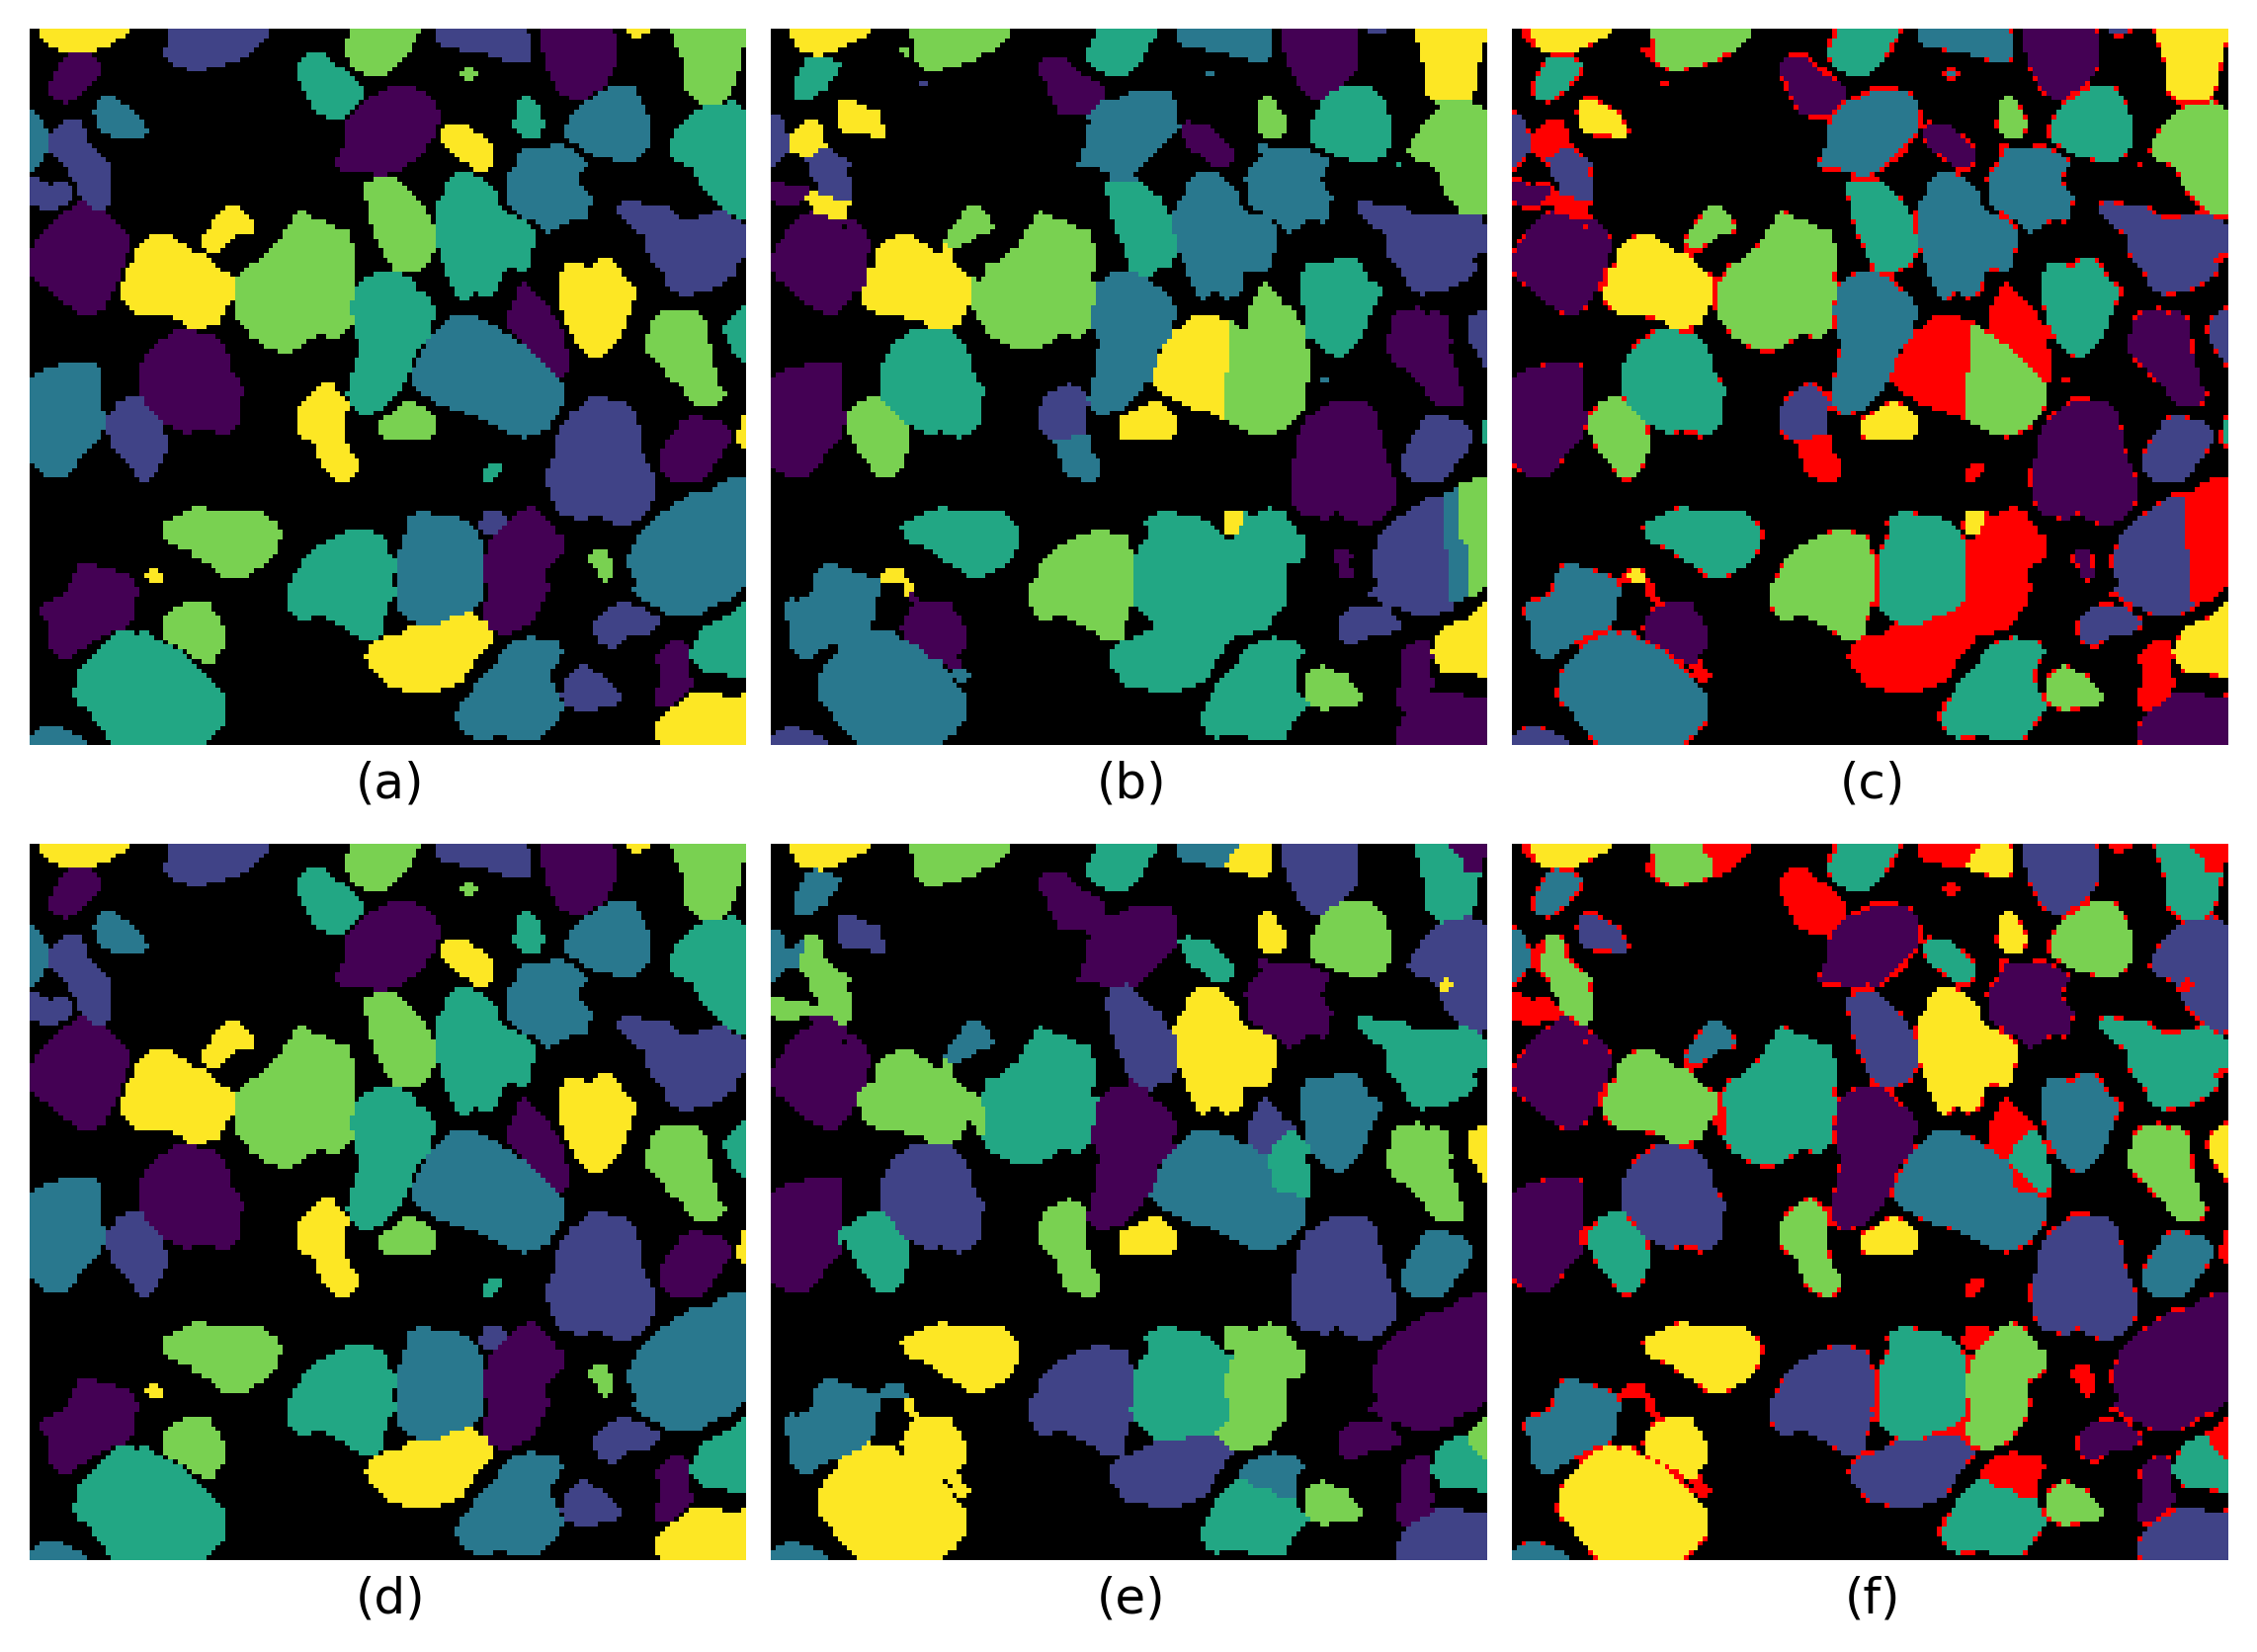
\includegraphics[width=0.75\textwidth]{figures/05/09-comps-to-manual.png}
    \caption{
        \small\setstretch{1}
        (a) Manual segmentation from hand drawing individual overlays
        on each visually discernible sand grain.
        (b) Typical watershed segmentation (\ref{fig/05/typical}).
        This segmentation achieves an 82.09\% match with the manual segmentation.
        (c) Watershed segmentation with red overlay depicting pixels mismatched
        from the manual segmentation.
        (d) Manual segmentation plotted again for ease of comparison with
        merged-region segmentation.
        (e) Merged-region segmentation from merging over-segmented
        neighboring regions without a separating edge
        (\ref{fig/05/merge-results}). This segmentation achieves an
        87.02\% match with the manual segmentation, approximately a 7\%
        improvement from the typical watershed segmentation.
        (f) Merged-region segmentation with red overlay depicting
        pixels mismatched from the manual segmentation.
    }
    \label{fig/05/seg-comps}
\end{figure}

The largest disagreement between the mismatch of the typical watershed
and merged-region segmentations is a cluster of sand grains at the bottom
center of each image. In the manual segmentation, the cluster is
identified as four large sand grains and one small sand grain. In the typical
watershed segmentation, the cluster is incorrectly identified as three sand
grains: the small sand grain, one large sand grain, and the final three large
sand grains identified as a single, larger grain. This is an example of
under-segmentation because the segmentation routine did not segment the sand
grains enough. The visualization of this
mismatch (\ref{fig/05/seg-comps}.c) also provides some insight to the
functioning of the mismatch calculation algorithm mentioned before, as the red
overlay classifies only two of the three large grains in the cluster as mismatched,
rather than all three. The third grain is classified as the matching portion of
the cluster because it is the largest constituent of the cluster and therefore
provides the highest number of overlapping pixels out of the three grains.
This same cluster of five particles is identified differently in the merged-region
segmentation. Each of the four large sand grains were
identified, but the small grain was identified as part of the rightmost
large sand grain. Even though the merged-region segmentation results are not
perfect for this cluster, misrepresenting the small sand grain results in
fewer mismatched pixels than the two larger mismatched grains in the typical
watershed segmentation.

The next largest mismatch disagreement between the typical
watershed and merged-region segmentation is a pair of tightly clustered sand
grains, one large and one medium sized, near the center of the image. In the
typical watershed segmentation, the grains are segmented into two regions, but
the segmentation occurs at the wrong location, leading to the entire small sand
grain identified as mismatching along with half of the large grain.
In the merged-region segmentation, the large sand grain is mostly segmented
correctly (aside from a small region near the boundary with the medium grain)
and the small sand grain is over-segmented into two regions instead of one.
Once again, the mismatch in the merged-region segmentation is less than that
of the typical watershed segmentation.

Another mismatch disagreement is in the segmentation of a large sand grain on the
lower right edge of the image. In the typical watershed segmentation, the grain
is over-segmented into three separate regions. The largest of these regions is
identified as matching with the manual segmentation, which leaves the two smaller
regions as mismatch. In the merged-region segmentation, the sand grain is correctly
identified as a single region. Contrasting this over-segmentation and directly below
this large grain in the bottom right corner is a pair of medium sand grains that are
improperly under-segmented as a single region in the typical watershed segmentation.
The two grains are segmented correctly in the merged-region segmentation, however,
with only a thin region of mismatch between the two grains.

Though the merged-region segmentation was calculated as more closely
matching the manual segmentation overall, there are still a few regions of
mismatch disagreement between the two segmentations where the typical watershed
routine yielded a segmentation that was closer to the manual segmentation
than the merged-region segmentation. The largest of these
regions is a pair of medium-sized grains in the top center of the image. While
these grains are properly segmented in the typical watershed segmentation, the
grains are under-segmented as a single region in the merged-region segmentation.
This leads to the smaller of these grains being identified as mismatching.
This kind of under-segmentation is also seen between a medium and small sand grain
in the upper left side of the merged-region segmentation, though this pair of sand
grains is also misrepresented in the typical watershed segmentation as four regions.
A similar example in which the merged-region segmentation under-segmented a small
sand grain occurred for a small sand grain between two larger grains in the bottom
left corner of the image. The sand grain was segmented separately in the typical
watershed segmentation, though even in that segmentation the surrounding
area was still identified as mismatching in a way reminiscent of the
merged-region segmentation.

There are also a few cases of over-segmented grains in the merged-region
segmentation that are not present in the typical watershed segmentation. The
largest of these is a medium sand grain in the bottom center of the image that
was improperly segmented into two regions. The rest of the over-segmented regions
in the merged-region segmentation (besides the over-segmentation of the smaller of
two tightly clustered sand grains previously mentioned) are around the edges of the
image (e.g., top left edge, top right edge, top right corner, bottom right edge).
These over-segmented regions are all rather small, so they don't contribute much to
the overall mismatch with the manual segmentation, but their presence raises the
question of whether this algorithm would be even more successful if it was applied
to an image that contained only complete particles not split by image borders.

The last features to note in these images are the portion of the red overlays
corresponding to thin regions around the edge of some sand grains. These pixels
correspond to small regions of mismatch where the footprints of the manual and
typical/merged-region segmentations do not agree. These mismatched areas are present
because both the typical watershed and merged-region segmentations require a semantic
segmentation step to create a binary image differentiating particles from background.
From this binary image, markers are generated and passed to the instance segmentation
portion of the routines to segment and label the individual particles. This process
is mostly the same for the typical watershed and merged-region segmentation, resulting in
similarly mismatched regions along the edges of the particles where the
semantic segmentation slightly differs from the footprint of the manual segmentation.
The reason these regions are only mostly the same for these segmentations is because the
process of selecting markers from each semantic segmentation is slightly different in the
merged-region segmentation versus the typical watershed, as described previously. This leads
to some of the smallest sand grains not receiving a marker in one segmentation, but receiving
a marker in the other, leading to discrepancies in the mismatch.
Regardless, these regions are small, so
their contributions to the larger mismatch of the image are minimal.

